\documentclass{llncs}

\usepackage{amsmath}
\usepackage{amssymb}
\usepackage{amscd}
\usepackage{txfonts}
\usepackage{amsfonts,semantic,colortbl,mathrsfs,stmaryrd}
\usepackage{epsfig,graphicx,subfigure}
\usepackage{enumerate,enumitem}
\usepackage{multirow,multicol}
\usepackage{tabularx}
\usepackage{linearA}
\usepackage{mathabx}
\usepackage{mathrsfs}

\newcommand{\act}[1]{{\xrightarrow{#1}{}}}
\newcommand{\Cao}{\underline{\mbox{\LinearACCCLXXXVI}}}
\newcommand{\Emp}{\underline{[]}}
\newcommand{\Lef}{\underline{[}}
\newcommand{\Rig}{\underline{]}}
\newcommand{\Gc}{{\mathcal{G}^{c}}}
\newcommand{\G}{\mathcal{G}}

\title{Bidirectional Transformation on Ordered Graphs}
\author{Fei Yang}
\institute
{ BASICS\\
  Department of Computer Science and Engineering\\
  Shanghai Jiao Tong University, P.R.China\\
  \email{iamyf@sjtu.edu.cn}
}

\begin{document}
\maketitle


\begin{abstract}
The linguistic (language-based) approach plays an important role in development of structured and well-behaved bidirectional transformations. It has been successfully applied to solve the callenging problem of bidirectional transformation on graphs, where a clear bidirectional semantics if given based on a bulk semantics of the structural recursion. However, the graphs that can be dealt with are limited to unordered ones, and it has not yet been known how to treat ordered graphs such as XML graphs in which the child nodes of a node are ordered. $\lambda_{FG}$ is a language for querying ordered graphs, a bulk semantics of structural recursion is provided for ordered graphs. In this paper, we show that ordered graphs can be bidirectionalized by a three-stage procedure. We provided a bidirectionalized procedure to eliminate $\epsilon$-edges. Further, a clear bidirectional semantics for transformation language $\lambda_{FG}$ can be defined. The key technical point is a novel way of bidirectionalizing the bulk semantics in $\lambda_{FG}$.
\end{abstract}

\keywords{Ordered Graphs, Bidirectional Transformation, Bulk Semantics, $\lambda_{FG}$ Language}

\section{Introduction}\label{sec:intro}

Bidirectional transformation provide a novel mechannism for sychronizing and maintaining the consistency of information between input and output. The are pervasive and has may potential applications, including the synchronization of replicated data in different formats, presentation-oriented structured document development, interactive user interface design, coupled software transformation, and the well-known \emph{view updating} mechanism which has been intensively studied in the database community.

The linguistic (language-based) approach gives a promising way for development of structured and well-behaved bidirectional transformation, in wich every expreesion simultaneously specifies both a forward and the responding (correct) backward transformation, and every composite of expressions defines a structured way of gluing smaller bidirectional transformations to a bigger one. Despite its usefulness for bidirectional transformation on lists and trees, it is a challenge to deal with bidirectional transformation on graphs. First, unlike lists and trees, there is no unique way of representing, constructing, or decomposing a general graph, and this requires a more precise definition of \emph{equivalence} between two graphs. Second, graphs have \emph{shared node and cycles}, which makes both forward and backward trasformation computation more complicated than that on trees; na\"{i}ve computation would visit the same nodes many times and possibly infinitely.

In our previous work, we challenged the probelm by showing that the linguistic approach can be applied to bidirectional transformation on graphs, where a cleawr bidirectional semantics is given for UnCAL, a graph algebra for the known graph query language UnQL. The key to this success is the bulk semantics of the structural recursion function a structural recursion is evaluated by first processing \emph{in parallel} on all edges of the input graph and then combining the results. This bulk semantics relies on introduction of $\epsilon$-edges to grapohs, providing a smart way of treating shared nodes and cycles in graphs and of tracing back from the view to the source.

However, the graphs that can be dealt with in this manner must be unorered. It has not yet been known how to treat ordered graphs such as XML graphs in which the child nodes of a node are ordered. One might consider encoding the ordered graphs in terms of unordered ones by introducing specialized edge labels, but this would make it difficult to keep consistency of these labels during transformation. In fact, it is an open problem, as pointed out in, how labels during tranformation on ordered graphs. In , a transformation language for ordered graph $\lambda_{FG}$ is provided, a bulk semantics for transformation on ordered graphs is also given. Thus, a natural question is how can we bidirectionalize transforamtion on ordered graphs via $\lambda_{FG}$.

In this paper, we show that the ordered graphs can be bidirectionalized. The work is based on the equivalence relation of bisimilarity and the query language $\lambda_{FG}$ on ordered graphs. The main technical contributions are three folds. First, a novel three-stage bidirectional transformation strategy is designed for ordered graphs. Next we give a bidirectionalized procedure to eliminate $\epsilon$-edges. Finally, we construct a bidirectional evaluation semantics for $\lambda_{FG}$. 

\section{Preliminaries}\label{sec:pre}

Ordered graphs is a graph model in which the branchings are ordered. We start from introducing a formal definition for ordered graphs, and give a bisimilarity equivalence relation on the ordered graphs.

\subsection{Ordered Graphs}\label{subsec:order-graph}

The graphs we treated here are multi-rooted, directed, and edge-labeled graphs with order on outgoing edges. This graph model has three prominent features: \emph{$\epsilon$-edges}, \emph{markers}, and \emph{graph concatenation}. An $\epsilon$-edges represents the a shortcut between two nodes, it is similar with the $\epsilon$-transition in automata. Markers can be treated as interfaces that connect the nodes to other graphs. A node can be marked with \emph{input} and \emph{output markers}. Graph concatenation sequentially aligns two graphs in a given order.

The ordered graph model is formally defined as follows. We write $\mathcal{L}$ for the set of \emph{labels} and $\mathcal{L}_{\epsilon}$ for $\mathcal{L}\cup\{\epsilon\}$. Let $X$ and $Y$ be finite sets of input and output markers; we add the prefix $\&$ for markers like $\& x$.
    An \emph{ordered graph} $G$ is defined by a triple $(V,B,I)$, where
    \begin{itemize}
        \item $V$ is the set of \emph{nodes},
        \item $B:V\rightarrow List(\mathcal{L}_{\epsilon}\times V+Y)$ is a \emph{branch function} mapping a node to a list of \emph{branches}: a branch in $\mathcal{L}_{\epsilon}\times V+Y$ is either a \emph{labeled edge} $\mathbf{Edge}(l,v)$ or an \emph{output marker} $\mathbf{Outm}\&y)$, and
        \item $I:X \rightarrow V$ is a function which determines the \emph{input nodes} (roots) of the graph.
    \end{itemize}

Here, every node in the range of $I$ is called a root. Note that a root node may have incoming edges. However, we can convert it to a equivalent graph having no such incoming edges.

We denote a graph with the input marker set $X$ and the output marker set $Y$ by $G^X_Y$. Moreover, we write $\G^X_Y$ to represent the set of such graphs. Another assumption is that the graphs we are going to talk about are restricted to finite graphs, which means the finiteness on the set of nodes. $\Gc^X_Y$ is used to denote the set of ordered graph with a countble width. It is obvious that the set of finite ordered graphs $\G^X_Y$ is a subset of $\Gc^X_Y$.

For the markers, we allow a graph to have multiple roots. When the graph is single-rooted, we often use $\&$ as the \emph{default marker} to indicate the root and use $\G_Y$ ot denote $G^{\{\&\}}_Y$. 

\subsection{Graph Constructors}\label{subsec:graph-constr}
\begin{figure}[ht]
	\centering
	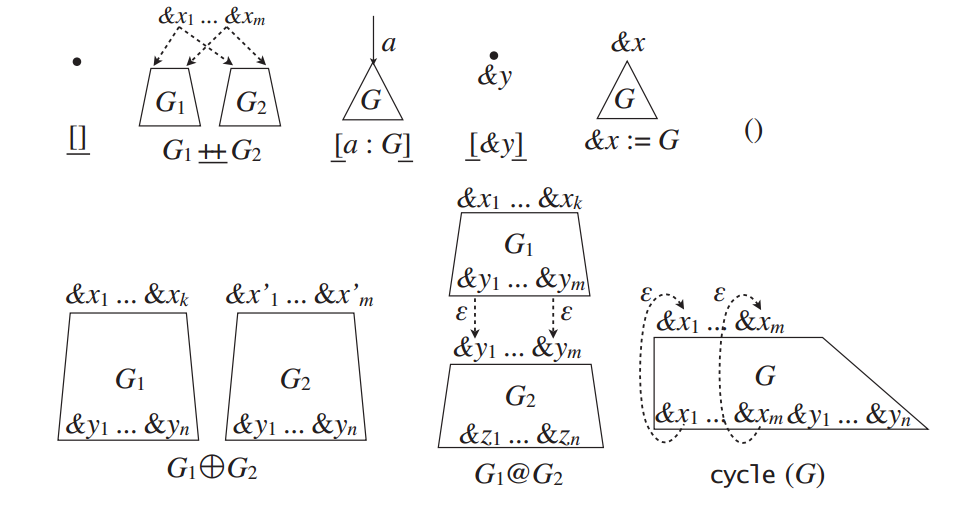
\includegraphics[width=0.8\textwidth]{fig1.png}
	\caption{Graph Constructors}
	\label{fig:graph-constr}
\end{figure}
Figure \ref{fig:graph-constr} sumarizes the nine costructors we used to describe arbitrary graphs.
$$\begin{array}{lcll}
G	&\Coloneqq	&\Emp	&\mbox{\{ single node graph \}}\\
	&\mid	&G_1\Cao G_2	&\mbox{\{ graph concatenation \}}\\
	&\mid	&\Lef a:G\Rig &\mbox{\{ an edge pointing to a graph \}}\\
	&\mid	&\Lef \&y\Rig &\mbox{\{ a node graph with an output marker \}}\\
	&\mid	&\&x\coloneqq G	&\mbox{\{ label he root node eith an input marker \}}\\
	&\mid	&()	&\mbox{\{ empty graph \}}\\
	&\mid	&G_1\oplus G_2	&\mbox{\{ disjoint graph union \}}\\
	&\mid	&G_1 @G_2	&\mbox{\{ append of two graphs \}}\\ 
	&\mid	&\mathbf{cycle}(G)	&\mbox{\{ graph with cycles \}}
\end{array}$$

The single node graph constructor $\Emp$ construct a root-only graph. $G_1\Cao G_2$ adds two $\epsilon$-edges from a new root to the roots of $G_1$ and $G_2$, respectively. $\Lef a:G\Rig$ constructs a graph adding an $a$ labeled edge point to the root of $G$. $\Lef\&y\Rig$ constructs a single node graph with an output marker $\&y$. $\&x\coloneqq G$ associates an input marker $\&x$ to the root node of $G$. $()$ constructs an empty graph with neither a node or an edge. Furthermore, $G_1\oplus G_2$ constructs a graph by using a componentwise $(V,B,I)$ union, $\Cao$ differs from $\oplus$ in that $\Cao$ unifies input nodes while $\oplus$ does not. $\oplus$ requires them to be identical. $G_1 @G_2$ composes two graphs by connecting the output nodes of $G_1$ with the corresponding input nodes of $G_2$ with $\epsilon$ edges. $\mathbf{cycle}(G)$ connects the output nodes of $G$ with the corresponding input nodes with $\epsilon$ edges, that will form cycles. The newly constructed nodes have unique identifiers. The formal definition of the sementics is given in $\lambda_{FG}$. 

\subsection{Proper Branches}\label{subsec:proper-b}

In the definition of ordered graphs, the $\epsilon$-edges are introduced to represent the shortcut between nodes. We need to relate two connected nodes by \emph{proper branch}, where we can ignore the shortcuts. A \emph{proper branch} of a node $v$ is defined as a path from $v$ going through zero or more $\epsilon$-edges until it reaches a non-$\epsilon$-edge or output marker.


Let $G=(V,B,I)\in\Gc^X_Y$ and $v\in V$. The path starting from $v$
$$v(=v_0)\act{\epsilon}_{i_0}v_1\ldots\act{\epsilon}_{i_{n-1}}v_n\act{}_{i_n}$$
is called a \emph{proper branch} of $v$ if the $i_n$-th branch $B(v_n).i_n$ is not an $\epsilon$-edge. (i.e. a non-$\epsilon$-edge or an output marker. The set of all proper branches of $v$ in $G$ is denoted by $Pb(G,v)$. 

Like the order on the branches, a total order is introduced on proper branches. Given two proper branches in an arbitrary graph, $p=(v\act{\epsilon}_{i_0}v_1\ldots\act{\epsilon}_{i_{n-1}}v_n\act{}_{i_n})$, and $p'=(v\act{\epsilon}_{i_0'}v_1'\ldots\act{\epsilon}_{i_{n'-1}'}v_{n'}'\act{}_{i_{n¡¯}'})$. Let their branch index sequences be $\tilde{p}\stackrel{def}{=}(i_0,\ldots,i_{n-1},i_n)$ and $\tilde{p'}\stackrel{def}{=}(i_0',\ldots,i_{n'-1}',i_{n'}')$. We define $p\leq_{Pb}p' \stackrel{def}{\Longleftrightarrow}\tilde{p}\leq_l\tilde{p'}$ where $\leq_l$ is the lexicographical order between branch index sequences. This order plays an important roll in the definition of bisimilarity and the procedure of bidirectionalizing elimination of $\epsilon$-edges.

For a given proper branch $p$, we use $p.last$ to denote the last step of the branch sequence, which is either a non-$\epsilon$ edge or a output marker.

\subsection{Bisimilarity for Ordered Graphs}\label{subsec:bis}

For the soundness of the graph model, we need an equivalence relation that can judge whether two arbitrary graphs are the same. At first glimpse, graph isomophism is the most straight forward approach. However, it is not necessarily that two graphs are isomophic when they behaves the same. Another option is language equivalence, which is focused on the language produced by the graphs, But unfortunately, it is proved to be undecidable in automata theory. Semantic equivalence is widely used in program verification to overcome the above difficulties. Bisimilarity is a kind of semantic equivalence, which is focused on the observable behavior of the graphs. 

On unordered graphs, we use the notion of value equivalence (Bisimilarity) as the equivalence relation used in verfication. A similar bisimilarity on ordered graphs is given.

For two graphs $G=(V,B,I)$and $G'=(V',B',I')$ in $\Gc^X_Y$, a relation $R$ between $V$ and $V'$ is called a \emph{bisimulation relation}, if for any $vRv'$, there is an order isomorphism $f:(Pb(G,v),\leq_{Pb})\rightarrow(Pb(G',v'),\leq_{Pb})$ satisfying he following order-preserving property: For any proper branch $p=(v\act{\epsilon}_{i_0}v_1\ldots\act{\epsilon}_{i_{n-1}}v_n\act{}_{i_n})\in Pb(G,v)$ with $f(p)=(v\act{\epsilon}_{i_0'}v_1'\ldots\act{\epsilon}_{i_{n'-1}'}v_{n'}'\act{}_{i_{n'}'})\in Pb(G',v')$, we have
\begin{itemize}
    \item Edge Correspondence: if $B(v_n).i_n=\mathbf{Edge}(l,u)$ for some $l\in\mathcal{L}, u\in V$, then  $\exists u'\in V'$ s.t. $B'(v_{n'}').i_{n'}'=\mathbf{Edge}(l,u')$ and $uRu'$,
    \item Marker Correspondence: if $B(v_n).i_n=\mathbf{Outm}(\&y)$ for some $\&y\in Y$, then $B'(v_{n'}').i_{n'}'=\mathbf{Outm}(\&y)$.
\end{itemize}
Two graphs $G$ and $G'$ are \emph{bisimilar} (denoted by $G\sim G'$) if there is a bisimulation relation $R$ s.t. for every input marker $\&x\in X$, $I(\&x)RI'(\&x)$.

The notion of bisimilarity only consider the reachable part of a given graph. This means the unreachable parts are disregarded, i.e. two bisimilar garphs are still bisimilar if one adds subgraphs unreachable frome input nodes.

\section{$\lambda_{FG}$: A Transformation Language for Ordered Graphs}\label{sec-lambda}

\subsection{The Core $\lambda_{FG}$}\label{subsec:core}

$\lambda_{FG}$ is a transformation language for transforming (querying) ordered graphs. There is a formal semantics for constructing and querying an ordered graph in $\lambda_{FG}$. It is an extenstion of typed $\lambda$-calculus with graph constructors and list functions. It has a powerful feature of structural recursion. It is capable of querying with manipulating the sibling of nodes, which gives a great expresiveness power to the language. The syntex of $\lambda_{FG}$ is given as below. It also has a system of strictly defined type inference rules.
$$\begin{array}{lclr}
\sigma	&\Coloneqq	&\sigma\rightarrow\sigma\mid\sigma+\sigma\mid\sigma\times\sigma	& \mbox{\{ function, coproduct, product types \}}\\
	&\mid	&\mathbf{List}(\sigma)\mid\mathbf{Bool} &\mbox{\{ list and boolean types \}}\\
	&\mid	&\mathbf{Label}\mid\mathbf{G}^X_Y	&\mbox{\{ label and graph types \}}\\
\\
e	&\Coloneqq	&x\mid\lambda x.e\mid e\,e\mid\mathbf{case}\,e\,\mathbf{of}\,\mathbf{in_l}(x)\rightarrow e\,\mathbf{or}\,\mathbf{in_r}(y)\rightarrow e	&\\
	&\mid	&\mathbf{in_l}e\mid\mathbf{in_r}e\mid(e,e)\mid\mathbf{pr_l}e\mid\mathbf{pr_r}e	&\mbox{\{ terms of lambda calculus \}}\\
	&\mid	&\mathbf{nil}\mid\mathbf{cons}(e,e)\mid\mathbf{foldr}(e,e)\mid\ldots &\mbox{\{ functions for lists \}}\\
	&\mid	&\mathbf{if}\,e\,\mathbf{then}\,e\,\mathbf{else}\,e	&\mbox{\{ conditional \}}\\
	&\mid	&a|e=e	& \mbox{\{ labels $(a\in\mathcal{L})$ and label equality \}}\\
	&\mid	&\Emp\mid e\Cao e\mid \Lef e:e\Rig\mid\Lef\&y\Rig\mid\&x\coloneqq e\mid()\mid e\oplus e	&\\
	&\mid 	&e @ e\mid \mathbf{cycle}(e)	&\mbox{\{ graph constructors \}}\\
	&\mid	&\mathbf{isEmpty}(e)	&\mbox{\{ graph emptiness checking \}}\\
	&\mid	&\mathbf{srec}(e,e)	&\mbox{\{ structural recursion functions \}}
\end{array}$$

Here we focus on the explaination of \emph{structural recursion}, which is a powerful graph transformation mechanism. It provides the capability to descirbe the queries and transformations that garantees the termination of the computation and preserves the finiteness.

In general the structure recursion is written of the form $\mathbf{srec}(e,d)$, wherer $e$ can be considered as the body function applied on the labeled edges and $d$ is a map computation on nodes. For a simple case, we can consider $d=\mathbf{foldr}(\odot,\iota_{\odot})$ for some monoid $(\odot,\iota_{\odot})$ on $\mathbf{G}^Z_{Z\times\alpha}$. The structural recursion function $f\stackrel{def}{=}\mathbf{srec}(e,d)$ satisfies the following equations (herer, equality means bisimilarity):
$$\begin{array}{lcl}
f(\Emp)	&=&	\iota_{\odot}\\
f(g_1\Cao g_2)	&=&	f(g_1)\iota f(g_2)\\
f(\Lef l:g\Rig)	&=&	e(l,g) @ f(g)\\
f(\&x\coloneqq g)	&=&	(\oplus_{\&z\in Z}(\&z,\&x)\coloneqq\Lef(\&z,\&\Rig)@f(g)\\
f(())	&=&	()\\
f(g_1\oplus g_2)	&=&	f(g_1)\oplus f(g_2)
\end{array}$$

\begin{example}\label{ex:a2dxc}
This example shows how to manipulate edges of the graph and change its shape by structural recursion, The following function $a2d\_xc$ replaces all labels $a$ with $d$ and contracts $c$-labeled edges. 
$$\begin{array}{lll}
a2d\_xc	&=\mathbf{srec}(rc,\mathbf{foldr}(\Cao,\Emp))&	\\
	&\mathbf{where}\,rc(l,g)=	&\mathbf{if}\,l=a\,\mathbf{then}\,\Lef d:\Lef\&\Rig\\
	&	&\mathbf{else}\,\mathbf{if}\,l=c\,\mathbf{then}\,\Lef\&\Rig\,\mathbf{else}\,\Lef l:\Lef\&\Rig\Rig
\end{array}$$
\end{example}

Compared with the structural recurcion in UnCAL, structural recurtion in $\lambda_{FG}$ can deal with orered graphs and computations on the sibling dimension of graphs. This ability is given by the function of $d$. 

\subsection{Bulk Semantics of Structural Recursion}\label{subsec:bulk}

The structural recursion of $\lambda_{FG}$ has two equivalent semantics. One is \emph{recursive semantics}. It defines the function behavior and the program transformation/optimization recursively. It appears to be more concise and is useful for reasoning. Another one is \emph{bulk semantics}. By allowing $\epsilon$-edges, we can evaluate a structural recursion in a \emph{bulk} manner. The bulk semantics consider the transformation on a whole. It is useful in parallel computation and the proof of termination and finiteness-preserving property. In the construction of bidirectional semantics, we will also apply the bidirectionlization on bulk semantics.

Before the introduction of bulk semantics, let us consider the type of the structural recursion function $\mathbf{srec}(e,d)$ in advance. A type inference rule is given below.

$$\inference{\vdash e:\mathbf{Label}\times\mathbf{G}_Y\rightarrow\mathbf{G}^Z_Z \vdash d:\mathbf{List}(\mathbf{G}^Z_{Z\times\alpha}+\mathbf{G}^Z_{Z\times Y})\rightarrow\mathbf{G}^Z_{Z\times\alpha+Z\times Y}}{\vdash\mathbf{srec}(e,d):\mathbf{G}^X_Y\rightarrow\mathbf{G}^{Z\times X}_{Z\times Y}}$$

Here, $e$ is the body function of the transformation on edges. it performs a similar role as the body function in the unordered version. It maps the a subgraph of a labeled edge into the result graph. For the $d$ function, it works as a rearrangement function over the lists. It maps the each lists by manipulate the order of the branches. In the bulk semantics, the evaluation can be applied in parallel. It mainly involves three steps.
\begin{enumerate}
	\item Map computation on edges with $e$: the function $e$ is applied on each labeled edge, yield a set of intermediate result graphs for $e$. The set graphs will be rearranged in the next step.
	\item Map computation on nodes with $d$: the function $d$ is applied on each nodes. The previous set of graphs are merged by the rearrangement measure defined in $d$, leads to a set of merged graphs for each node.
	\item Groups new graphs with $\epsilon$-edges: to get the final result, the graphs for each node need to be grouped by $\epsilon$-edges. The $\epsilon$-edges are added according to the input and output markers of the previous result. 
\end{enumerate}

\section{An Overview of Bidirectional Transformation}\label{sec:overview}

In UnCAL, there is a framework that could bidirectionalize unordered graph transformation. It consists of a two stage bidirectionalizing strategy and it could solve the problem that the graphs may contain shared nodes or cycles. This framework provides us a some heuristic idea to do the bidirectionalizing on $\lambda_{FG}$. 

The challenging parts of bidirectionalizing on $\lambda_{FG}$ comes from the $d$ function in the structural recursion. It leads to a three step bulk semantics, which would make it hard to trace back from the view. Further, the $d$ function only accepts graphs without $\epsilon$-edges. Thus, an $\epsilon$-elimination procedure has to be applied before the structural recursion for an arbitrary graph. Also, the $\epsilon$-edge should be eliminated before it is presented to the customer. Moreover, the order of the branchings must be treated carefully in our bidirectionalization. 

\subsection{Bidirectional Properties}\label{subsec:b-prop}

The goal in bidirectionalizing $\lambda_{FG}$ is to approach the bidirectionalization in ordered graphs by providing a bidirectional semantics in $\lambda_{FG}$. The semantics should have bidirectional properties defined in the previous work in UnCAL. Let $\mathscr{F}\ldbrack e\rdbrack\rho$ denote a forward evaluation (get) of expression $e$ under environment $\rho$ to produce a view, and $\mathscr{B}\ldbrack e\rdbrack(\rho,G')$ denote a backward evaluation (put) of expression $e$ under environment $\rho$ to reflect a possibly modified view $G'$ to the source by computing an updated environment. An \emph{environment} $\rho$ is a mapping with a form $\{\$x\mapsto X,\ldots\}$ where $X$ is a graph $G$ or a label $l$, and $\$x$ is a variable. The transformation need to satisfy the following two important properties:

$$\inference{\mathscr{F}\ldbrack e\rdbrack\rho=G}{\mathscr{B}\ldbrack e\rdbrack(\rho,G)=\rho}(GETPUT)\quad
\inference{\mathscr{B}\ldbrack e\rdbrack(\rho,G')=\rho' \mathscr{F}\ldbrack e\rdbrack\rho'=G''}{\mathscr{B}\ldbrack e\rdbrack(\rho,G'')=\rho'}(WPUTGET)$$

The (GETPUT) property states that unchanged view $G$ should give no change on the environment $\rho$ in the backward evaluation, while the (WPUTGET) property states that the modified view $G'$ and the view obtained by backward evaluation followed by forward evaluation may differ, but both view have the same effect on the original source if backward evaluation is applied. A pare of forward and backward evaluation is \emph{well-behaved} if it satisfies (GETPUT) and (WPUTGET) proties. In the rest of the paper, the forward and backward evaluations will be presented for $\lambda_{FG}$, and the following theorem holds.

\begin{theorem}[Well-behavedness]\label{th:wellb}
The proposed forward and backward evaluations are well-behaved, provided their evaluations succeed.
\end{theorem}

According to the (WPUTGET) property, given a certain forward evaluation function, there could be more than one backward evaluation that would satisfy the well-behavedness property. When we perform the modification on the view, the most reasonable choice is to reflet it on the corresponding part on the source. This is the \emph{location correspondence} property. Moreover, the modification on the view graph could be categorised into three types: in place updates, edge deletion and edge insertion. In order to maintain the well-behavedness between the updated source and the modified view, we also need to apply some operation on the source. A reasonable assumption is that a certain type of modification on the view yields the same type of operation on the source, which could be called the \emph{operation correspondence} property. We say this kind of reflection on updates are rational.

%\begin{theorem}[Rationality]\label{th:rat}
%The proposed bidirectional transformation on $\lambda_{FG}$, satisfies both location and operation correspondence property. We call it a rational transformation.
%\end{theorem}

The rationality property is also important as it gives us a discriptive goal in designing the bidirectionalizing the transformation. The goal is to let the updates on the source to meet the intention of the changing on the view.

\subsection{Three-Stage Bidirectionalization}\label{subsec:3-sta}

In an arbitrary transformation, there could be a big gap between the source and view graoh. It makes it hard to reflect changes on the view to the source. The basic idea to divide the forward evaluation into three stages, each one could be bidirectionalized.
\begin{itemize}
	\item Stage 1: Elimination of $\epsilon$-edges on the source, to produce a simple source that we can apply bulk semantics on it.
	\item Stage 2: Forward evaluation using bulk semantics. This stage may create some new $\epsilon$-edges, so that the output graph will have a similar shape to the input graph. Appropriate trace information might be appended locally on the nodes in the result graph.
	\item Stage 3: Elimination of $\epsilon$-edges to produce a usual view.
\end{itemize}

In our bidirectional transformation framework, we will propose a general bidirectionalized $\epsilon$-edge elimination procedure for both Stage 1 and Stage 3. For Stage 2, a bidirectionalized semantics for $\lambda_{FG}$ is provided in this paper. Thus, the whole transformation is bidirectionlized by a inductively defined procedure.

\section{Bidirectionalizing $\epsilon$-elimination procedure}\label{sec:eps}

In the previous work of $\lambda_{FG}$, the input graph of the $d$ function in structural recursion does not accept any $\epsilon$-edges. However, we can not safely assume that an arbitrary input graph does not contain any $\epsilon$-edges. Further, after applying the transformation via bulk semantics, some $\epsilon$-edges might be introduced to maintain the structure of the result graph. In most applications, $\epsilon$-edges are assumed to be unobservable. Thus, we wish to produce a view without any $\epsilon$ to the users. In this seciton, a bidirectionalized $\epsilon$-elimination procedure is proposed. 

First, there is an effective procedure that whether the $\epsilon$-elimination could be applied successfully on a finte ordered graph $G$. The details could be found in the paper of $\lambda_{FG}$.

\begin{lemma}\label{lamma:eps-exists}
Given an finite ordered graph $G$ possibly with $\epsilon$-edges, there is an effective procedure to decide whether there exists an ordered graph $G'$, s.t. $G\sim G'$ and has neither $\epsilon$-edges nor infinite width. If yes, produce such $G'$.
\end{lemma}

The idea of the $\epsilon$-elimination procedure is to use labeled edges to connect the shortcut between proper branches, the procedure is defined as below. Note that we use a list of integers to represent the total orders over the branches and proper branches on a node.

\begin{definition}\label{def:epsilon}
For a graph $G=(V,B,I)\in\Gc^X_Y$, the $\epsilon$-elimination $\epsilon\mbox{-elim}(G)$ of $G$ is a graph $(V,B'I)\in\Gc^X_Y$ where $|B'(v)|\stackrel{def}{=}Pb(G,v)$, and $B'(v).\tilde{p}\stackrel{def}{=}Pb(G,v).\tilde{p}.last$ for $p=(v\act{\epsilon}_{i_0}\ldots v_n\act{}_{i_n})$ in $B'(v)$.
\end{definition}

Next we will introduce how to reflect view updates within $\epsilon\mbox{-elim}(G)$ to the source graph $G$. We will use the correspondence between the proper branches in the source graph and the branches in the view graph.

\begin{enumerate}
	\item For the inplace-updates on an arbitrary edge $B'(v).\tilde{p}\in\epsilon\mbox{-elim}(G)$, the corresponding labeled edge on the view is $Pb(G,v).\tilde{p}.last$. We could apply the same update operation on this edge. 
	\item For the edge deletion on an arbitrary edge $B'(v).\tilde{p}\in\epsilon\mbox{-elim}(G)$, we update the source graph by delete the correcponding edge $Pb(G,v).\tilde{p}.last$.
	\item For the edge insertion, since the set of nodes $V$ is the same on the view and the source. Thus, we just need to insert the edge to the same place on the source.
\end{enumerate}

After we have done the update operation on the source, an $\epsilon$-elimination procedure need to be applied again on the updated source. The reason is that, the updated labeled edge may be duplicated in different proper branches. Thus, the corresponding edge of these proper branches on the view graph also need to be updated to mainain the consistency between the source and the view. For inplace updates and edge deletion, the corresponding edge is deleted on the view, and for edge insertion, the edge is added according to the newly added proper branches. Therefore, the whole procedure would satisfy the well-behavedness. Moreover, the rationality is also infered from this constructive bidirectionalizing procedure.

\begin{lemma}\label{lemma:well-epsilon}
The proposed bidirectionalized $\epsilon$-elimination procedure satisfy the well-behavedness and the rationality property.
\end{lemma}

\section{Traceble Forward Evaluation}\label{sec:fwd}

Practically, a $\lambda_{FG}$ expression usually specifies a forward transformation that maps a source ordered graph (possibly a database or an XML file) to a view graph. A backward transformation for this procedure specifies how to reflect view updates to the source graph. However, the structural information kept by $\epsilon$-edges will not appear explicitely in the view graph. Moreover, the newly created parts within the transformation procedure also make it hard to detect the generated source for everything in the view graph. In this sence, some appropriate trace information should be added to the view, to make the view more informative, in other words, \emph{traceable}. In this section, we will enrich the original semantics of $\lambda_{FG}$ to make it produces traceable view after forward transformation.

\subsection{Local Trace Information}\label{subsec:local}

Recall the semantics in $\lambda_{FG}$, a view is obtained by evaluating a $\lambda_{FG}$ expression with an ordered graph. Every node in the view graph is either a graph obtained from the source graph, or a node constructed by te $\lambda_{FG}$ expression, except the node generated through a structural recursion(in bulk semantics). For an arbitrary structural recursion function $\mathbf{srec}(e_1,d)(e_2)$, the input of the body function $e_1$ is evaluated binding variables from a part of evaluated result in $e_2$; and the input of the rearrangement $d$ function is evaluated by binding variables from the result in $e_1$. So the node in the result graph may originate from not only the whole $srec$ expression but also a sub-expression in $e_2$. Thus, a more complicated inductively defined trace information should be added on the nodes on the result graph.

Here, we use the a \emph{traceable view} in which each node has information for tracing its origin. This locally added information, called $TraceID$, is defined by

$$\begin{array}{lll}
TraceID &\coloneqq	&SrcID\\
	&\mid		&Code\,Pos\,Marker\\
	&\mid		&RecN\,Pos\,TraceID\,Marker\\
	&\mid		&RecE\,Pos\,TraceID\,TraceID\,Num\\
	&\mid		&RecM\,Pos\,Marker\,TraceID\,Num\\
	&\mid		&RecD\,Pos\,TraceID\,TraceID
\end{array}$$

Where $SrcID$ ranges over the identifiers uniquely assigned to all nodes in the source graph, $Pos$ ranges over code positions in the $\lambda_{FG}$ expressions, $Marker$ ranges over input/output makers, and Num ranges over the lists of integers, which represent the order of the branches. 

Now we briefly expain the meaning of each $TraceID$. $SrcID$ means the node is generated from the corresponding one in the source. $Code\,Pos\,Marker$ is the information for the nodes created by the $\lambda_{FG}$ expreesion on the marked code position. $RecN,\,RecE,\,RecM,\,RecD$ are four kinds of trace information used in bidirectionalizing structural recursion $\mathbf{srec}(e,d)$. $RecN\,RecE\,RecM$ represent the node in the intermediate result after $e$ is applied, which are generated from the nodes/edges/markers respectively, and $RecD$ information is added when the rearrangements on the lists are applied by $d$. 

\subsection{Enriched Forward Semantics}\label{subsec:fwd-sem}

Now we will define the enriched forward semantics of $\lambda_{FG}$ that could generate a traceable view. Recall the core of $\lambda_{FG}$ language introduced in \ref{subsec:core}, the tracing information is recorded when a node is created. Let $e^p$ denote an $\lambda_{FG}$ subexpression $e$ at code position $p$. We write $\rho(\$x)$ for $G$ when $(\$x\mapsto G)\in\rho$, and $e\rho$ means the variable substitution using $\rho$ in the expression $e$. We inductively define the enriched forward semantics $\mathscr{F}\ldbrack e^p\rdbrack\rho$ for each $\lambda_{FG}$ construct of $e$.

In addition, we replace the composition of markers in $X\times Z$ by a monoid $(.,\&)$, with $\&$ as the identity, i.e., $\&.\&x=\&x.\&=\&x$. In particular, $\{\&\}.Z=Z.\{\&\}=Z$ for any $Z$. We call ``$.$'' the Skolem function.
 
\textbf{Graph Constructor Expressions} The semantics of graph constructor expressions is straightforward according to the construction in Fig\ref{fig:graph-constr}. For instance, the enriched semantic of single node graph constructor is,

$\mathscr{F}\ldbrack\Emp^p\rdbrack\rho=(\{Code\, p\},\{Code\, p\mapsto[]\},\{\&\mapsto Code\, p\})$

Note that the code position is added in the node, which infers that it is generated by the expression of in position $p$. Moreover, the branch set is nonempty despite there is no edge in the graph.

As another example, the semantics for the expression $e_1\Cao e_2$ is defined below. Note that there is no such combinator in unordered version for that it remains the order of the graphs when it links the input markers.

$\mathscr{F}\ldbrack (e_1\Cao e_2)^p\rdbrack\rho=\mathscr{F}\ldbrack e_1\rdbrack\rho\Cao^p\mathscr{F}\ldbrack e_2\rdbrack\rho$\\
$\mbox{~~~~}\mathbf{let}\,G_1\Cao^p G_2=(V_1\cup V_2\cup V',B_1\cup B_2\cup B',I')$\\
$\mbox{~~~~~}\mathbf{where}\,(V_1,B_1,I_1)=G_1,\,(V_2,B_2,I_2)=G_2$\\
$\mbox{~~~~~~~}M=\mathbf{inMarker}(G_1)=\mathbf{inMarker}(G_2)$\\
$\mbox{~~~~~~~}V'=\{Code\,p\,\&m\mid\&m\in M\}$\\
$\mbox{~~~~~~~}B'=\{Code\,p\,\&m\mapsto[\mathbf{Edge}(\epsilon,I_1(\&m)),\mathbf{Edge}(\epsilon,I_2(\&m))]\mid \&m\in M\}$\\
$\mbox{~~~~~~~}I'=\{\&m\mapsto Code\,p\,\&m\mid\&m\in M\}$

where $\Cao^p$ is a union operator for two graphs concerning position $p$. We write $\mathbf{inMarker}(G)$ and $\mathbf{outMarker}(G)$ to denote the set of input and output markers in a graph $G$, respectively.

$e_1\oplus e_2$ is a componentwise union operator like $\Cao$, exept that no $\epsilon$-edges are involved.

$\mathscr{F}\ldbrack(e_1\oplus e_2)^p \rdbrack\rho=\mathscr{F}\ldbrack e_1\rdbrack\rho\oplus\mathscr{F}\ldbrack e_2\rdbrack\rho$\\
$\mbox{~~~~}\mathbf{let}\,G_1\oplus G_2=(V_1\cup V_2,B_1\cup B_2,I_1\cup I_2)$\\
$\mbox{~~~~~~}\mathbf{where}\,(V_1,B_1,I_1)=G_1;(V_2,B_2,I_2)=G_2$

For the empty graph constructor and constant marker graph, it is easy to define

$\mathscr{F}\ldbrack()^p \rdbrack\rho=(\{\},\{\},\{\})$\\


$\mathscr{F}\ldbrack\Lef \&m\Rig^p\rdbrack\rho=(\{Code\,p\},\{Code\,p\mapsto[\mathbf{Out}m(\&m)]\},\{\&\mapsto Code\,p\})$

The next two constructors append labeled edges and markers with a graph respectively.

$\mathscr{F}\ldbrack\Lef l:e\Rig^p\rdbrack\rho=(\{Code\,p\}\cup V,\{Code\,p\mapsto[(l\rho,I(\&))]\}\cup B,\{\&\mapsto Code\,p\})$\\
$\mbox{~~~~}\mathbf{where}\,(V,B,I)=\mathscr{F}\ldbrack e\rdbrack\rho$\\

TraceID is generated for the newly constructed node.

$\mathscr{F}\ldbrack(\&m\coloneqq e)^p\rdbrack\rho=(\&m\coloneqq \mathscr{F}\ldbrack e\rdbrack\rho)$\\
$\mbox{~~~~}\mathbf{let}\,(\&m\coloneqq G)=(V,B,I')$\\
$\mbox{~~~~~~}\mathbf{where}\,(V,B,I)=G$\\
$\mbox{~~~~~~}I'=\{\&m.\&x\mapsto v\mid(\&x\mapsto v)\in I\}$

Here ``$.$'' is the Skolem function introduced before.

$e_1@ e_2$ appends two graphs by connecting the output nodes of the left operand and corresponding input nodes of the right operand with $\epsilon$-edges.

$\mathscr{F}\ldbrack(e_1@ e_2)^p \rdbrack\rho=\mathscr{F}\ldbrack e_1\rdbrack\rho\, @^p\mathscr{F}\ldbrack e_2\rdbrack\rho$\\
$\mbox{~~~~}\mathbf{let}\,G_1@^pG_2=(V_1\cup V_2,B_1'\cup B_2,I_1)$\\
$\mbox{~~~~~~}\mathbf{where}\,(V_1,B_1,I_1)=G_1,\,(V_2,B_2,I_2)=G_2$\\
$\mbox{~~~~~~}B_{1}'=\{u\mapsto\left[
	\begin{array}{lll}
	x.i	&=\mathbf{Edge}(l,v)	&\Rightarrow x.i\\
		&=\mathbf{Outm}(\&m)	&\Rightarrow (\epsilon,I_2(\&m))
	\end{array}\right]_{i\in |x|}\mid (u\mapsto x)\in B_1\}$

$\mathbf{cycle}(e)$ is defined as follows

$\mathscr{F}\ldbrack(\mathbf{cycle}(e))^p \rdbrack\rho=\mathbf{cycle}^p(\mathscr{F}\ldbrack e \rdbrack\rho)$\\
$\mbox{~~~~}\mathbf{let}\,\mathbf{cycle}^p(G)=(V,B',I)$\\
$\mbox{~~~~~~}\mathbf{where}\,(V,B,I)=G$\\
$\mbox{~~~~~~}B'=\{u\mapsto\left[
	\begin{array}{lll}
	x.i	&=\mathbf{Edge}(l,v)	&\Rightarrow x.i\\
		&=\mathbf{Outm}(\&m)\wedge\&m\in dom(I)		&\Rightarrow \mathbf{Edge}(\epsilon,I(\&m))\\
		&=\mathbf{Outm}(\&m)\wedge\&m\notin dom(I)	&\Rightarrow x.i
	\end{array}\right]_{i\in |x|}\mid (u\mapsto x)\in B\}$

\textbf{Labels} In $\lambda_{FG}$ the type of labels and boolean is strictly defined. The forward semantics for label and label equality are

$\mathscr{F}\ldbrack a^p\rdbrack\rho=\quad a\rho\quad(a\in\mathcal{L})$

$\mathscr{F}\ldbrack (l_1=l_2)^p\rdbrack\rho=\quad l_1\rho=l_2\rho$

\textbf{Variables} The query of ordered graph via $\lambda_{FG}$ requries the variable abstraction and application operations. The forward semantics for variable looks up its binding environment $\rho$ is.

$\mathscr{F}\ldbrack(\$v)^p\rdbrack\rho=\rho(\$v)$

\textbf{Condition} The forward semantics of a condition is defined as

$\mathscr{F}\ldbrack (\mathbf{if}\,e_1\,\mathbf{then}\,e_2\,\mathbf{else}\,e_3)^p\rdbrack\rho=\left\{
    \begin{array}{ll}
     \mathscr{F}\ldbrack e_2\rdbrack\rho& \mathbf{if}\,\mathscr{F}\ldbrack e_1\rdbrack\rho\\
     \mathscr{F}\ldbrack e_3\rdbrack\rho& otherwise
    \end{array}
    \right.$

It first evaluates the conditional expression $e_1$, and with the result it chooses the right branch to evaluate.

\textbf{Emptiness Checking} The forward semantics of emptiness checking function is defined as

$\mathscr{F}\ldbrack(\mathbf{isEmpty}(e))^p\rdbrack\rho=\mathbf{isEmpty}(\mathscr{F}\ldbrack e\rdbrack\rho)$

\textbf{Function on Lists} For the function on the lists, here we consider it as a polymorphism on the nodes for simplicity, There is a formal way of bidirectionalizing the node polymorohism, which is done by previous work. So we will not include the details.

\textbf{Structural Recursion} The forward semantics of a structural recursion in $\lambda_{FG}$ is given by \emph{bulk semantics}. It can be formally defined by three stages:

$\mathscr{F}\ldbrack (\mathbf{srec}(e_b,d)(e_a))^p\rdbrack\rho=G_{srec}$\\
\mbox{~~~~}$\mathbf{let}\,G=\mathscr{F}\ldbrack e_a\rdbrack\rho,\quad Z=Marker(e_b)$\\
\mbox{~~~~~~}$\mathbf{where}\,(V,B,I)=G\,(G\mbox{ has no }\epsilon\mbox{-edges}),\quad G|_v=(V,B,\{\&\mapsto v\})$
\begin{enumerate}
\item First apply edge mappings using $e$.

\mbox{~~~~}$B_v=\{u\mapsto\left[
    \begin{array}{ll}
    x.i=\mathbf{Edge}(l_i,v_i)& \Rightarrow (\mathscr{F}\ldbrack e_b\rdbrack\rho_{u,i},v_i)\\
    &\quad\rho_{u,i}=\rho\cup\{\$l\mapsto l_i,\$g\mapsto G|_{v_i}\}\\
    x.i=\mathbf{Out}m(\&y) & \Rightarrow x.i
    \end{array}\right]_{i\in|x|}|(u\mapsto x)\in B\}$

Then use $RecN,\,RecE,\,RecM$ to mark the nodes within the graph generated by the nodes, edges and markers respectively,

$V_{RecE_{u,i}}=\{RecE\,p\,w\,u\,i|(u\mapsto x)\in B_v,\,i\in|x|,\,x.i=(G_{u,i},v),\,w\in G_{u,i}.V\}$\\
$\mbox{~~~~~~}B_{RecE_{u,i}}=\{RecE\,p\,w\,u\,i\mapsto\left[
    \begin{array}{ll}
    x'.j=\mathbf{Edge}(l_j,w_j)& \Rightarrow \mathbf{Edge}(l_j,RecE\,p\,w_j\,u\,i)\\
    x'.j=\mathbf{Out}m(\&m) & \Rightarrow \mathbf{Out}m(\&m,\&RecN\,p\,v\,\&m)
    \end{array}\right]_{j\in |x'|}|(u\mapsto x)\in B_v,\,i\in|x|,\,x.i=(G_{u,i},v),\,(w\mapsto x')\in G_{u,i}.B,\,\&m\in Z\}$\\
$\mbox{~~~~~}I_{RecE_{u,i}}=\{\&m\mapsto RecE\,p\,w\,u\,i|(u\mapsto x)\in B_v,\,i\in|x|,\,x.i=(G_{u,i},v),\,(\&m\mapsto w)\in G_{u,i}.I\}$

$V_{RecM_{u,i}}=\{RecM\,p\,\&m\,u\,i|(u\mapsto x)\in B_v,\,i\in |x|,\, x.i=\mathbf{Out}m(\&y),\,\&m\in Z\}$\\
$\mbox{~~~~~}B_{RecM_{u,i}}=\{RecM\,p\,\&m\,u\,i\mapsto [\mathbf{Out}m(\&m,\&y)]|(u\mapsto x)\in B_v,\,i\in |x|,\, x.i=\mathbf{Out}m(\&y),\,\&m\in Z\}$\\
$\mbox{~~~~~}I_{RecM_{u,i}}=\{\&m\mapsto RecM\,p\,\&m\,u\,i|(u\mapsto x)\in B_v,\,i\in|x|,\,x.i=\mathbf{Out}m(\&y),\,\&m\in Z\}$

$V_{RecN}=\{RecN\,p\,v\,\&m|v\in V\,\&m\in Z\}$\\
$\mbox{~~~~}B_{RecN}=\{RecN\,p\,u\,\&m\mapsto\left[
    \begin{array}{ll}
    x.i=(G_{u,i},v)& \Rightarrow (V_{RecE_{u,i}},B_{RecE_{u,i}},I_{RecE_{u,i}})\\
    x.i=\mathbf{Out}m(\&y) & \Rightarrow (V_{RecM_{u,i}},B_{RecM_{u,i}},I_{RecM_{u,i}})
    \end{array}\right]_{i\in |x|} |u\in V,\,(u\mapsto x)\in B_v,\,\&m\in Z\}$

\item Then apply node mapping using $d$.

$G_{d_v}=\mathscr{F}\ldbrack d_v\rdbrack\rho_{d_v}$\\
$\mbox{~~~~}\mathbf{where}\,v\in V_{RecN},\quad\rho_{d_v}=\{\$b\mapsto B_{RecN}(v)\}$

\item We add $RecD$ information on the result graphs and merge them by $\epsilon$-edges.

$V_{RecD_v}=\{RecD\,p\,u\,v|v\in V_{RecN},\,u\in G_{d_v}.V\}$\\
$\mbox{~~~~}B_{RecD_v}=\{RecD\,p\,u\,v\mapsto\left[
    \begin{array}{ll}
    x.i=\mathbf{Edge}(l_i,w_i)& \Rightarrow \mathbf{Edge}(l_i,RecD\,p\,w_i\,v)\\
    x.i=\mathbf{Out}m(\&m,\&v') & \Rightarrow \mathbf{Edge}(\epsilon,I_{RecD_v}(\&m,\&v'))\\
    x.i=\mathbf{Out}m(\&m,\&y) & \Rightarrow x.i
    \end{array}\right]_{i\in |x|}|v\in V_{RecN},\,(u\mapsto x)\in G_{d_v}.B,\,\&m\in Z,\,v'(\neq v)\in V_{RecN}\}$\\
$\mbox{~~~~}I_{RecD_v}=\{(\&m,\&v)\mapsto RecD\,p\,u\,v|v\in V_{RecN},\,\&m\in Z,\,u=G_{d_v}.I(\&m)\}$\\
$\mbox{~~~~}I_{RecD}=\{(\&m,\&y)\mapsto u|\&m\in Z,\,\&y\in Dom(I),\,v=I(\&y),\,v'=RecN\,p\,v\,\&m,\,u=I_{RecD_{v'}}(\&m,\&v')\}$

The final result is

$G_{srec}=(\bigcup_{v\in V_{RecN}}V_{RecD_v},\bigcup_{v\in V_{RecN}}B_{RecD_v},I_{RecD})$

\end{enumerate}
\section{Backward Evaluation}\label{sec:bak}

Thanks to the bulk semantics in $\lambda_{FG}$ and the trace information generated at enriched forward evaluation, the similarity in shape between input and output graphs are retained. As in previous work of unordered graph, the graph constructors become invertible, and the backward evaluation $\mathbf{rec}(e,d)$ is reduced to that of its body $e$ and $d$. We again devide backward evaluation algorithm by updates supported: (1) edge-renaming, (2) edge-deletion, and (3) insertion of edges or a subgraph rooted at a node. In the following, we give the backward semantics for these updates.

\subsection{Reflection of Inplace Updates}\label{subsec:bak-inp}

Backward semantics is, similarly to the forward semantics, defined inductively, i.e. backward evaluation of a $\lambda_{FG}$ expression is computed by combining results of backward evaluations of the operand expressions. We first define backward semantics of the simple expressions, followed by that of structural recursion.

\textbf{Graph Constructor Expressions} 

In order to merge the environment computed by the inductively defined,backward evaluation, we need a to define a merge operator.

$\rho_1 \uplus_{\rho}\rho_2=\left\{(x\mapsto\mathbf{mg}(G,G_1,G_2)
    \begin{array}{|l}
     (x\mapsto G_1)\in\rho_1\\
     (x\mapsto G)\in\rho\\
     (x\mapsto G_2)\in\rho_2
    \end{array}
    \right\}$

$\mathbf{where}\,\mathbf{mg}(G,G_1,G_2)=\left\{
\begin{array}{ll}
    G_1 & \mathbf{if}\,G_2=G\vee G_1=G_2\\
    G_2 & \mathbf{if}\,G_1=G\\
    FAIL & otherwise
\end{array}\right.$

$\Emp$, $\&y$ and $()$ construct constant graphs in the forward computation. Therefore, for the backward computation, they accept no modification on the view.

$\mathscr{B}\ldbrack \Emp^p\rdbrack(\rho,G')=\rho\quad if\,G'=\mathscr{F}\ldbrack \Emp^p\rdbrack\rho$\\
$\mbox{~~~~~}\mathscr{B}\ldbrack \Lef\&m\Rig^p\rdbrack(\rho,G')=\rho\quad if\,G'=\mathscr{F}\ldbrack \Lef\&m\Rig^p\rdbrack\rho$\\
$\mbox{~~~~~}\mathscr{B}\ldbrack ()^p\rdbrack(\rho,G')=\rho\quad if\,G'=\mathscr{F}\ldbrack ()^p\rdbrack\rho$

$\Lef l:e\Rig$ backward computation detaches (possibly modified) edge from the top of the modified graph. Other modification on the graph is reflected to the other operand $G_2$ (as $G_2'$)

$\mathscr{B}\ldbrack \Lef l:e\Rig^p\rdbrack(\rho,G')=\mathscr{B}\ldbrack l\rdbrack(\rho,a')\uplus_{\rho}\mathscr{B}\ldbrack e\rdbrack(\rho,G_2')$\\
$\mbox{~~~~}\mathbf{where}\,a=l\rho$\\
$\mbox{~~~~~~~~~~~~~~}G_2=\mathscr{F}\ldbrack e\rdbrack\rho$\\
$\mbox{~~~~~~~~~~~~~~}(a',G_2')=decomp_{\Lef a:^p G_2\Rig}(G')$

Here, the decompositon function is defined as follows

$decomp_{\Lef a_1:^p G_2\Rig}(G')=\mbox{~~~~}(a_1',(V'\setminus\{r'\},B'\setminus\{r'\mapsto\zeta'\},\{\&\mapsto v\}))$\\
$\mbox{~~~~}\mathbf{where}\,(V_2,B_2,\{\&\mapsto v\})=G_2$\\
$\mbox{~~~~~~~~~~~~~~~} (V',B',\{\&\mapsto r'\})=G'$\\
$\mbox{~~~~~~~~~~~~~~~}\zeta'=\,the\,unique\,branch\,in\,B'\,of\,the\,form\,([\mathbf{Edge}(a_1',v)])$.

The modified view $G'$ is decomposed into its unique root branch $\zeta'=[\mathbf{Edge}(a_1',v)]$ from the original root $r'$ and  the rest of the graph rooted at $v$. If $G'$ has more than one branches from the root node or the new root $v$ does not match the root node of the original result $G_2$, the backward evaluation fails.

$e_1\Cao e_2$ We have the following definition ,given $decomp_{G_1\Cao G_2)}(G')$ as the decomposition of the graph $G'$

$\mathscr{B}\ldbrack (e_1\Cao e_2)^p\rdbrack(\rho,G')=\mathscr{B}\ldbrack e_1\rdbrack(\rho,G_1')\uplus_{\rho}\mathscr{B}\ldbrack e_2\rdbrack(\rho,G_2')$\\
$\mbox{~~~~}\mathbf{where}\,G_1=\mathscr{F}\ldbrack e_1\rdbrack\rho$\\
$\mbox{~~~~~~~~~~~~~~~~}G_2=\mathscr{F}\ldbrack e_2\rdbrack\rho$\\
$\mbox{~~~~~~~~~~~~}(G_1',G_2')=decomp_{G_1\Cao^p G_2}(G')$
    
$decomp$ is defined as below. $G_1\setminus G_2$ denotes $(V_1\setminus V_2,B_1\setminus B_2,I_1\setminus I_2)$ where $B_1\setminus B_1$ and $I_1\setminus I_2$ respectively denote removal of bindings in $B_2$ and $I_2$ from those in $B_1$ and $I_1$. Simple union of graphs $G_1\cup G_2$ is defined be $(V_1\cup V_2, B_1\cup B_2, I_1\cup I_2)$.

$decomp_{G_1\Cao^p G_2}(G')=(xreachable(G_1'',G_1),xreachable(G_2'',G_2))$\\
$\mbox{~~~~}\mathbf{where}\,(V',B',I')=G'\quad(V_i,B_i,I_i)=G_i$\\
$\mbox{~~~~~~~~~~~~~~~} G_i''=reachable((V',B',I_i))$\\
$\mbox{~~~~}\mathbf{satisfying}\,M=Dom(I_1)=Dom(I_2)$\\
$\mbox{~~~~~~~~~~~~~~~}\forall\&m\in M,\,\mathbf{Edge}(\epsilon,v')\in B'(I'(\&m)): (\&m\mapsto v')\in I_1\cup I_2$ \\
$\mbox{~~~~}unreachable(G)=G\setminus reachable(G)$\\
$\mbox{~~~~}xreachable(G'',G)=reachable(G'')\cup unreachable(G)$

$e_1\oplus e_2$ It is like $Cao$, except no $\epsilon$-edge is involved.

$\mathscr{B}\ldbrack (e_1\oplus e_2)^p\rdbrack(\rho,G')=\mathscr{B}\ldbrack e_1\rdbrack(\rho,G_1')\uplus_{\rho}\mathscr{B}\ldbrack e_2\rdbrack(\rho,G_2')$\\
$\mbox{~~~~}\mathbf{where}\,G_1=\mathscr{F}\ldbrack e_1\rdbrack\rho$\\
$\mbox{~~~~~~~~~~~~~~~}G_2=\mathscr{F}\ldbrack e_2\rdbrack\rho$\\
$\mbox{~~~~~~~~~~~~~~~}(G_1',G_2')=decomp_{G_1\oplus^p G_2}(G')$\\
$\mbox{~~~~~~~~~~~~~~~}decomp_{G_1\oplus^p G_2}(G')=(xreachable(G_1'',G_1),xreachable(G_2'',G_2))$\\
$\mbox{~~~~~~~~~~~~~~~}\mathbf{where}\,(V',B',I')=G'\quad(V_i,B_i,I_i)=G_i$\\
$\mbox{~~~~~~~~~~~~~~~~~~~~~~~~~~~} G_i''=reachable((V',B',I_i))$

It is the same as $decomp_{G_1\Cao^pG_2}(G')$ without $\mathbf{satisfying}$ condition.

$e_1 @e_2$ Because of unmatched I/O nodes, it may introduce unreachable part in the second argument during forward computation. Backward computation carefully passes those parts backwards untouched to avoid unnecessary failure because of inconsistency, and these parts are part of ordinary computation (computation on reachable parts) before discarding by the $@$ operator.

$\mathscr{B}\ldbrack (e_1@ e_2)^p\rdbrack(\rho,G')=\mathscr{B}\ldbrack e_1\rdbrack(\rho,G_1')\uplus_{\rho}\mathscr{B}\ldbrack e_2\rdbrack(\rho,G_2')$\\
$\mbox{~~~~}\mathbf{where}\,G_1=\mathscr{F}\ldbrack e_1\rdbrack\rho$\\
$\mbox{~~~~~~~~~~~~~~~}G_2=\mathscr{F}\ldbrack e_2\rdbrack\rho$\\
$\mbox{~~~~~~~~~~~~~~~}(G_1',G_2')=decomp_{G_1@^p G_2}(G')$

$decomp_{G_1@^p G_2}(G')=(xreachable(G_1'',G_1),xreachable(G_2'',G_2))$\\
$\mbox{~~~~}\mathbf{where}\,(V',B',I')=G'\quad(V_i,B_i,I_i)=G_i$\\
$\mbox{~~~~~~~~~~~~~~~}B''=\{ u\mapsto\left[
    \begin{array}{ll}
    x.i=\mathbf{Edge}(\epsilon,v)\wedge u\in V_1 &\\
    \wedge B_1(u).i=\mathbf{Out}m(\&m)&\\
    \wedge (\&m\mapsto v)\in I_2 & \Rightarrow \mathbf{Out}m(\&m)\\
    otherwise & \Rightarrow x.i
    \end{array}\right]_{i\in|x|}|(u\mapsto x)\in B'\}$\\
$\mbox{~~~~~~~~~~~~~~~}G_i''=reachable((V',B'',I_i))$

$\&m\coloneqq e$ It ``peels off'' the marker on the left hand side from each of the input markers in $G'$ at the front.

$\mathscr{B}\ldbrack(\&m\coloneqq e)^p\rdbrack(\rho,G')=\mathscr{B}\ldbrack e\rdbrack(\rho,G_1')$\\
$\mbox{~~~~}\mathbf{where}\,(V',B',I')=G'$\\
$\mbox{~~~~~~~~~~~~~~~}I_1'=\{(\&x\mapsto v)|(\&m.\&x\mapsto v)\in I'\}$\\
$\mbox{~~~~~~~~~~~~~~~}G_1'=(V',B',I_1')$

 $\mathbf{cycle}(e)$ It removes the $\epsilon$-edges introduced in the forward evaluationo and restores the original output markers.

$\mathscr{B}\ldbrack(\mathbf{cycle}(e))^p\rdbrack(\rho,G')=\mathscr{B}\ldbrack e\rdbrack(\rho,G_2')$\\
$\mbox{~~~~}\mathbf{where}\,(V',B',I')=G'\quad(V,B,I)=\mathscr{F}\ldbrack e\rdbrack\rho$\\
$\mbox{~~~~~~~~~~~~~~~} B_{cycle}=\{ u\mapsto\left[
    \begin{array}{ll}
    x.i=\mathbf{Edge}(\epsilon,v)&\\
    \wedge B(u).i=\mathbf{Out}m(\&m)& \Rightarrow \mathbf{Out}m(\&m)\\
    otherwise & \Rightarrow x.i
    \end{array}\right]_{i\in|x|}|(u\mapsto x)\in B'\}$\\
$\mbox{~~~~~~~~~~~~~~~} G_2'=(V,B_{cycle},I)$

\textbf{Labels} A label constant and label equality accepts no modification.

$\mathscr{B}\ldbrack a\rdbrack(\rho,a')=\rho\quad\mathbf{if}\,a'=a$

$\mathscr{B}\ldbrack (l_1=l_2)\rdbrack(\rho,e')=\rho\quad\mathbf{if}\,e'=\mathscr{F}\ldbrack (l_1=l_2) \rdbrack\rho$

\textbf{Variables} A variable simply updates its bindings as $\mathscr{B}\ldbrack\$ v\rdbrack(\rho,G')=\rho[\$v\leftarrow G']$. Here, $\rho[\$v\leftarrow G']$ is an abbreviation for $(\rho\setminus\{\$v\mapsto\_\})\cup\{\$v\mapsto G'\}$.

\textbf{Condition} A backward evaluation of a condition is defined by

$\mathscr{B}\ldbrack (\mathbf{if}\,e_1\,\mathbf{then}\,e_2\,\mathbf{else}\,e_3)\rdbrack(\rho.G')=\left\{
    \begin{array}{ll}
     \rho_2'& \mathbf{if}\,\mathscr{F}\ldbrack e_1\rdbrack\rho\wedge\mathscr{F}\ldbrack e_1\rdbrack\rho_2'\\
     \rho_3'& \mathbf{if}\,\neg\mathscr{F}\ldbrack e_1\rdbrack\rho\wedge\neg\mathscr{F}\ldbrack e_1\rdbrack\rho_3'\\
     FAIL & otherwise
    \end{array}
    \right.$\\
$\mbox{~~~~}\mathbf{where}\,(\rho_2',\rho_3')=(\mathscr{B}\ldbrack e_2\rdbrack(\rho,G'),\mathscr{B}\ldbrack e_3\rdbrack(\rho,G'))$

which is reduced to the backward evaluation of $e_2$ if $e_1$ holds and to the backward evaluation of $e_3$ otherwise. To guarantee well-behavedness, we further ensure the boolean expression $e_1$ does not change after backward evaluation. Because the result of $e_1$ may be influenced indirectly by backward evaluation of the bodies $e_2$ and $e_3$, if they update variable bindings and the value of variables in the condition is produced from the updated bindings, and check that condition at the expression binding the variables. However, to simplify presentation, we omit this passing around of conditions and checkings in the following.

\textbf{Emptiness} A backward evaluation of an emptiness checking is defined by

$\mathscr{B}\ldbrack\mathbf{isEmpty}(e)\rdbrack(\rho,e')=\rho\quad\mathbf{if}\,e'=\mathscr{F}\ldbrack \mathbf{isEmpty}(e)\rdbrack\rho$

As the reason explained before, we simply does not allow the change of boolean values in the backward evaluation.

\textbf{Structural Recursion} Backward evaluation of a structural recursion function is defined by the following stepwise procedure. It performs the inverse procedure of the forward evaluation. The most crucial point is to use the trace information of structural recursion to decompose the view graph into subgraphs before adding the $\epsilon$-edges. Further, when we merge the updated environment, we first merge local changes, then merge it to the whole changes. Since there might be overlapped parts among theng, we let the backward evaluation fails if the overlapped parts are inconsistant. The backward evaluation of the body expression can be inductively defined.

$\mathscr{B}\ldbrack \mathbf{srec}(e_b,d)(e_a)\rdbrack(\rho,G_{srec}')=\rho'$\\
$\mbox{~~~~}\mathbf{where}\,(V_{srec}',B_{srec}',I_{srec}')=G_{srec}'$
\begin{enumerate}
\item We first decompose the result graph into subgraphs by the trace information on $RecD$ functions. 

$\mbox{~~~~}V_{d_v}'=\{u|v\in V_{RecN},\,(RecD\,p\,u\,v)\in V_{srec}'\}$\\
$\mbox{~~~~}B_{d_v}'=\{u\mapsto\left[
    \begin{array}{ll}
    x.i=\mathbf{Edge}(l_i,RecD\,p\,w_i\,v)& \Rightarrow \mathbf{Edge}(l_i,w_i)\\
    x.i=\mathbf{Edge}(\epsilon,I_{RecD_v}(\&m,\&v')& \Rightarrow \mathbf{Out}m(\&m,\&v'))\\
    x.i=\mathbf{Out}m(\&m,\&y) & \Rightarrow x.i
    \end{array}\right]_{i\in |x|}|v\in V_{RecN},\,((RecD\,p\,u\,v)\mapsto x)\in B_{srec}',\,\&m\in Z,\,v'(\neq v)\in V_{RecN}\}$\\
$\mbox{~~~~}I_{d_v}'=\{\&m\mapsto u|v\in V_{RecN},\,\&m\in Z,\, RecD\,p\,u\,v\in Range(I_{RecD_v})\}$\\
$G_{d_v}'=(V_{d_v}',B_{d_v}',I_{d_v}')$

\item Then apply the backward evaluation of function $d$ on each subgraph. Applying decomposition on the result using the trace information of $RecE$ and $RecD$.

$\rho_{d_v}'=\mathscr{B}\ldbrack d_v\rdbrack(\rho_{d_v},G_{d_v}')$\\
$\mbox{~~~~}V_{u,i}'=\{v|u\in V,\,(RecN\,p\,u\,\&m\mapsto x)\in \rho_{d_{RecN\,p\,u\,\&m}}'(\$b),\,i\in |x|,%\,x.i.I(\&m)=(RecE\,p\,w\,u\,i),
\,(RecE\,p\,v\,u\,i)\in x.i.V,\,\&m\in Z\}$\\

$\mbox{~~~~}B_{u,i}'=\{v\mapsto\left[
    \begin{array}{ll}
    x'.j=\mathbf{Edge}(l_j,RecE\,p\,v_j\,u\,i)& \Rightarrow \mathbf{Edge}(l_j,v_j)\\
    x'.j=\mathbf{Out}m(\&m,\&(RecN\,p\,u'\,\&m)) & \Rightarrow \mathbf{Out}m(\&m)\\
    \end{array}\right]_{j\in |x'|}|u\in V,\,(RecN\,p\,u\,\&m\mapsto x)\in \rho_{d_{RecN\,p\,u\,\&m}}'(\$b),\,i\in |x|,
    %\,x.i.I(\&m)=(RecE\,p\,w\,u\,i),\,
    \,((RecE\,p\,v\,u\,i)\mapsto x')\in x.i.B\}$\\
$\mbox{~~~~}I_{u,i}'=\{\&m\mapsto w|u\in V,\,(RecN\,p\,u\,\&m\mapsto x)\in \rho_{d_{RecN\,p\,u\,\&m}}'(\$b),\,i\in |x|,\,x.i.I(\&m)=(RecE\,p\,w\,u\,i)\}$\\
$G_{u,i}'=(V_{u,i}',B_{u,i}',I_{u,i}')$

\item Apply the backward evaluation of $e$. Finally, reconstruct the updated view.

$\rho_{u,i}'=\mathscr{B}\ldbrack e_b\rdbrack(\rho_{u,i},G_{u,i}')$\\
%%$\mathbf{where}\, VV_{u,i}\neq\emptyset$\\
$G'=(V'\cup\bigcup\rho_{v,i}'(\$g).V,B'\cup\bigcup\rho_{v,i}'(\$g),B,I)$\\
$\mbox{~~~~}\mathbf{where}\,V'=\{\{v\}\cup\{w|Edge(l,w)\in s\}|(v\mapsto s)\in B'\}$\\
$\mbox{~~~~~~~~~~~~~~~}B'=\{v\mapsto \left[
    \begin{array}{ll}
    x.i=\mathbf{Edge}(l_i,v_i)& \Rightarrow \mathbf{Edge}(\rho_{v,i}'(\$l),v_i)\\
    x.i=\mathbf{Out}m(\&m) & \Rightarrow x.i\\
    \end{array}\right]_{i\in |x|}|(v\mapsto x)\in B\}$\\
$\rho'=\mathscr{B}\ldbrack e_a\rdbrack(\rho,G')\uplus_{\rho}\biguplus\{\rho_{v,i}'\setminus\{\$\mapsto\_\}\setminus\{\$g\mapsto\_\}\}$

\end{enumerate}

\subsection{Reflection of Edge Deletion}\label{subsec:bak-del}

Similarly to the treatment in the previous work, we reflect deletion of an edge in the view as deletion of corresponding edge int eh source using trace IDs. In unordered graph, edge is identified by the triple of origin node, label and destination node, but here we can identify with a pair of origin node and branch position.

$corr$ defined below takes a pair of origin node ID and branch position that uniquely identify an edge in the view, and computes the corresponding edge as a pair of origin node ID and branch position in the source.

$corr((u,i))=(u,i)\quad if\, u\in SrcID$\\
$\mbox{~~~~~~}corr((RecE\,p\,u\,v\,i,j))=\left\{
		\begin{array}{ll} 
			corr((u,j)) & if\,corr((u,j))\neq FAIL\\
			corr((v,i)) & if\,corr((u,j))= FAIL
		\end{array}\right.$\\
$\mbox{~~~~~~}corr((RecD\,p\,u\,v,j))=corr((u,j))$\\
$\mbox{~~~~~~}corr(\zeta)=FAIL\quad otherwise$

$FAIL$ means failure on finding the corresponding edge.

Note that only labeled edges are allowed to be deleted in the view. Thus, the nodes with trace information $RecN$ and $RecM$ will never appear in the input of $corr$.

Using this function, we compute the set of corresponding edges from set of deleted edges on the updated view $G_{view}'$. If one of the computation $corr$ fails, then the backward evaluation fails. Otherwise, we compute the updated source $G_{src}'$ by removal of the set of corresponding edges (branches). Note that we use the list of integers as the branch number, thus the relative position the following (sibling) branches will not change if we delete one edge.

Finally, get the updated view $G_{view}''=\mathscr{F}\ldbrack e\rdbrack\rho[\$g\rightarrow G_{src}']$ in order to keep the consistancy of the well-behavedness between updated source and view. Moreover, we need to check if this updated view is bisimilar to the changed view $G_{view}'$.

The (WPUTGET) property is straight forward, since our final check actually will promise that. Thus the backward transformation on edge deletion is also well-behaved.

\subsection{Reflection of Edge Insertion}\label{subsec:bak-ins}

The method used in previous work of handling insertion in unordered graph can be adopted here.

The insertion operation on the view is specified by a triple of a node $v$ on the view and the position $i$ where a graph is inserted, and the inserted graph $G_{vins}$. Then we first compute the corresponding source node $u$ at which insertion of corresponding subgraph $G_{sins}$ takes plase, by the following function $tr$.

$tr(SrcID)=SrcID\quad tr(RecN\,\_\,v\,\_)=tr(v)$

$tr(Code\,\_\,\_)=FAIL\quad tr(RecE\,\_\,v\,\_\,\_)=tr(v)$

$tr(RecD\,\_\,v\,\_\,\_)=tr(v)\quad tr(RecM\,\_\,\_\,\_\,\_)=FAIL$

We find a graph $G_{sins}$ connected to $u$ and the corresponding position $j$ at which $G_{sins}$ is connected ,by inversion computation on $G_{view}'$ using the Universal Resolving Algorithm (URA), wherer $G_{view}'$ is obtained by adding $\epsilon$-edge from $v$ at position $i$ to $G_{vins}$.

We conjecture that well-behavedness of the above insertion reflection can be directly derived from the soundness of URA.

\subsection{Well-Behavedness}

Now, according to the inductive way of building the bidirectional semantics, we have the well-behavedness property.

\begin{proof}
For the bidirectional evaluation semantics, this statement can be proved by induction on the structural of expression $e$, in a way similar to that in unordered graph. Note that we perform aggressive check for branch changing behavior of \textbf{if} for this well-behavedness. Further, the bidirectionalization of $\epsilon$-elimination procedure is also well-behaved. Thus Theorem\ref{th:wellb} is proved.
\end{proof}

\section{Conclusion}\label{sec:con}

In this paper, we give a way of bidirectionalizing the transformation on ordered graphs. A three-stage bidirectionalizing strategy is provided, and we proved that each stage could be bidirectionalized. 


\end{document}
